%\documentclass[handout]{rsuqbeamernew}
\documentclass{rsuqbeamernew}
\def\ANIMATE{0}   %   0/1: Compile animations or not

%%%%%%%%%%%%%%%%%%%%%%%%%%%%%%%%%%%%%%%%%%%%%%%%%%%%%%%%%%%%%%%%%%%%%%%%%%%%%%%%%%%%%%%%%%%%%%%%%%%%%%
%
%
%
\title[HPC Meeting]{Dispatcher Restart}
\subtitle{HPC Meeting}
\institute[Chair of Risk \& Safety] {}
\author[D. Wicaksono]{Damar Wicaksono}

\date[December 03, 2019] {\small December 03, 2019}

% graphics
\graphicspath{{Figures/},{Figures/Christos/}}

\usepackage{bstnotations}
\usepackage[noend]{algpseudocode}
\usepackage{algorithm}
\usepackage{animate}
\usepackage{listings}

\definecolor{matlabComment}{rgb}{0.13,0.55,0.13}
\lstset{language=Matlab,
  basicstyle=\lstbasicfont\upshape\scriptsize,
  keywordstyle=\color{blue},
  numberstyle=\tiny,
  frame=shadowbox,rulesepcolor=\color{gray},
  commentstyle=\lstbasicfont\scriptsize\upshape\bf\color{matlabComment},
  breaklines=false,
  showstringspaces=false,
  morekeywords={uqlab,uq_retrieveSession,uq_create_xyz, 
    uq_createInput,uq_createModel,uq_createAnalysis,
    uq_createDispatcher,uq_set_workflow,UQ_input,
    UQ_model,UQ_analysis,UQ_dispatcher,
    UQ_workflow,UQ, uq_runAnalysis, uq_runAnalysis,
    uq_create_hpc_dispatcher,
    uq_retrieveSession,uq_get_model_response,
    uq_calculateMetamodel, uq_getSample,
    uq_enrichSample,uq_default_input,
    uq_enrichLHS, uq_enrichSobol, uq_enrichHalton, uq_LHSify,
    uq_evalModel, uq_runModel, uq_runAnalysis,
    uq_selectInput,uq_selectAnalysis,uq_selectModel,uq_select_xyz,
    uq_getInput,uq_getAnalysis,uq_getModel,
    uq_setDefaultSampling,uq_GeneralIsopTransform,uq_IsopTransform,
    uq_sampleU,
    uq_NatafTransform, uq_invNatafTransform, uq_MarginalFields,
    uq_print, uq_display
  },
  xleftmargin=0.03\textwidth,
  xrightmargin=0.03\textwidth,
  aboveskip=2mm,
  belowskip=2mm,
  tabsize=1,
  %    linewidth=\textwidth,
  literate={~} {$\sim$}{1}
}

% additional
\newcommand{\card}[1]{\mathrm{card}(#1)}
\DeclareMathOperator*{\argmax}{arg\,max}
\DeclareMathOperator*{\argmin}{arg\,min}

% algorithm abbreviations
\newcommand{\Ntot}{\textsc{Ntot}}
\newcommand{\Ninit}{\textsc{Ninit}}
\newcommand{\M}{\textsc{M}}
\newcommand{\Nneigh}{\textit{NNeighbour}}
\newcommand{\NBound}{\textsc{NBoundaries}}
\newcommand{\NneighThresh}{\textsc{NNeighbourThreshold}}
\newcommand{\Penal}{\textit{Penalization}}
\newcommand{\Pmax}{\textsc{Pmax}}
\newcommand{\NRefine}{\textsc{NRefine}}
\newcommand{\NRefineIter}{\textsc{NEnrIter}}
\newcommand{\Func}[1]{\textsc{model}(#1)}
\newcommand{\Inp}[1]{\textsc{input}(#1)}
\newcommand{\X}{\textit{X}}
\newcommand{\Xcurr}{\textit{Xcurr}}
\newcommand{\Xnew}{\textit{Xnew}}
\newcommand{\Y}{\textit{Y}}
\newcommand{\Ycurr}{\textit{Ycurr}}
\newcommand{\Ynew}{\textit{Ynew}}
\newcommand{\PCEref}{\textit{PCEpar}}
\newcommand{\Dref}{\textit{Dpar}}
\newcommand{\Di}{\textit{Di}}
\newcommand{\Dcand}{\textit{Dcand}}
\newcommand{\Dfirst}{\textit{D1}}
\newcommand{\Dsec}{\textit{D2}}
\newcommand{\Dnew}{\textit{Dchild}}
\newcommand{\Res}{\textit{Resid}}
\newcommand{\Rescurr}{\textit{ResidualCurr}}
\newcommand{\Errors}[1]{\textit{Errors}#1}
\newcommand{\ErrorLoo}{\textit{ErrorLOO}}
\newcommand{\Domain}[1]{\textit{Domains}#1}
\newcommand{\PCEs}[1]{\textit{PCEs}#1}
\newcommand{\PCEnew}{\textit{PCEchild}}
\newcommand{\RefineDom}[1]{{\altx \textsc{getRefineDomain}}(#1)}
\newcommand{\ConstrPCE}[1]{{\altx \textsc{constructPCE}}(#1)}
\newcommand{\EnrExpD}[1]{\textsc{enrichDesign}(#1)}
\newcommand{\ConstrSSE}[1]{\textsc{constructSSE}(#1)}
\newcommand{\Size}[1]{\textsc{getSize}(#1)}
\newcommand{\Volume}[1]{\textsc{getVolume}(#1)}
\newcommand{\EvalSSE}[1]{\textsc{evaluateSSE}(#1)}
\newcommand{\ComputeError}[1]{\textsc{estimateError}(#1)}
\newcommand{\SplitDomain}[1]{{\altx \textsc{splitDomain}}(#1)}
\newcommand{\SelectRefine}[1]{{\altx \textsc{selectRefine}}(#1)}
\newcommand{\degC}{\ensuremath{\,^{\circ}\mathrm{C}}}
\newcommand{\BParams}{1}
\newcommand{\Bparams}{1}
\newcommand{\Bprior}{1}
\newcommand{\Bcond}{1}
\newcommand{\Bevi}{1}

% algorithm environment
\algnewcommand{\Inputs}[1]{%
	\State \textbf{inputs:}
	\vspace{-1em}
	\Statex \hspace*{\algorithmicindent}\parbox[t]{0.96\linewidth}{\raggedright 
		#1}
}
\algnewcommand{\Repeater}[1]{%
	\State \textbf{repeat:}
	\vspace{-1em}
	\Statex \hspace*{\algorithmicindent}\parbox[t]{0.96\linewidth}{\raggedright 
		#1}
}

\algnewcommand{\Initialize}[1]{%
	\State \textbf{initialize:}
	\vspace{-1em}
	\Statex \hspace*{\algorithmicindent}\parbox[t]{0.96\linewidth}{\raggedright 
		#1}
}


%%%%%%%%%%%%%%%%%%%%%%%%%%%%%%%%%%%%%%%%%%%%%%%%%%%%%%%%%%%%%%%%%%%%%%%%%%%%%%%%%%%%%%%%%%%%%%%%%%%%%%
\begin{document}

%----------------------------------------------------------------------------------------------------
\begin{frame}[t]{Dispatcher}
  \small

  \Tit{Pre-requisites for parallel computations}:
  \begin{itemize}
    \item Parallelized algorithm/functions/modules
    \item Parallel computing resources (hardware)
    \item Required information (e.g., about computing resources) to conduct parallel computations
  \end{itemize}

  \begin{block}{Dispatcher unit}
    A Dispatcher unit is a support object that {\altx contains} the information and {\altx performs} some IT operations required to conduct parallel computations, be it locally or in a remote cluster, of parallel algorithms or functions in \uqlab.
  \end{block}
  
  \Tit{Dispatcher-aware}
  
  \begin{itemize}
    \item[] {\altx Dispatcher-aware} functions (or modules) in \uqlab{} are functions (resp. modules) that support parallel computation using the information stored in a Dispatcher unit. How a particular module, function, or algoritm is parallelized is defined out of the Dispatcher unit itself.
  \end{itemize}

% If a parallelization of a function can be exploited, then module developers should simply conform with the interface provided by the Dispatcher unit for the actual parallel computation.
% A dispatcher unit should provide the interface such that a parallel algorithm can access the computing resources to conduct parallel computation.
\end{frame}

%----------------------------------------------------------------------------------------------------
%----------------------------------------------------------------------------------------------------
\section{Dispatcher-aware function}
\secoutline


%----------------------------------------------------------------------------------------------------
\begin{frame}[fragile,t]{\texttt{uq\_evalModel}: a Dispatcher-aware function}
	\small

  \Tit{\mcode{uq_evalModel}}
  \begin{itemize}
    \item If a Dispatcher unit is not specified (\emph{i.e.,} empty) then the evaluation is done locally on a single CPU\footnote{\matlab{} has a built-in support for multi-threaded computation for some functions.}.
    \item To create a Dispatcher unit, define a Dispatcher configuration options and a remote cluster profile, and create a Dispatcher unit.
    \item Call the function with an \mcode{'HPC'} flag.
  \end{itemize}

\begin{lstlisting}
%% Define a Dispatcher and remote cluster profile (i.e., credential)
...
uq_createDispatcher(DispatcherOpts) 
%% Evaluate Y = f(X) in parallel
Y = uq_evalModel(X,'HPC');  % HPC flag (use the Dispatcher unit)
\end{lstlisting}

  \emphconc{The execution of a parallel computation for \mcode{uq_evalModel} is {\altx transparent} to user. Be it local or in cluster, the user just get the Y values as requested; other than specifying a Dispatcher unit and using the flag, users will see no other difference.}
\end{frame}

%----------------------------------------------------------------------------------------------------
\begin{frame}[t]{\texttt{uq\_evalModel} and SSH Dispatcher unit in action}
  \small
   \only<1>{
    \includegraphics[width=0.95\textwidth]{ssh_dispatcher-first_step}
  }
  \only<2>{
    \includegraphics[width=0.95\textwidth]{ssh_dispatcher-second_step}
  }
  \only<3>{
    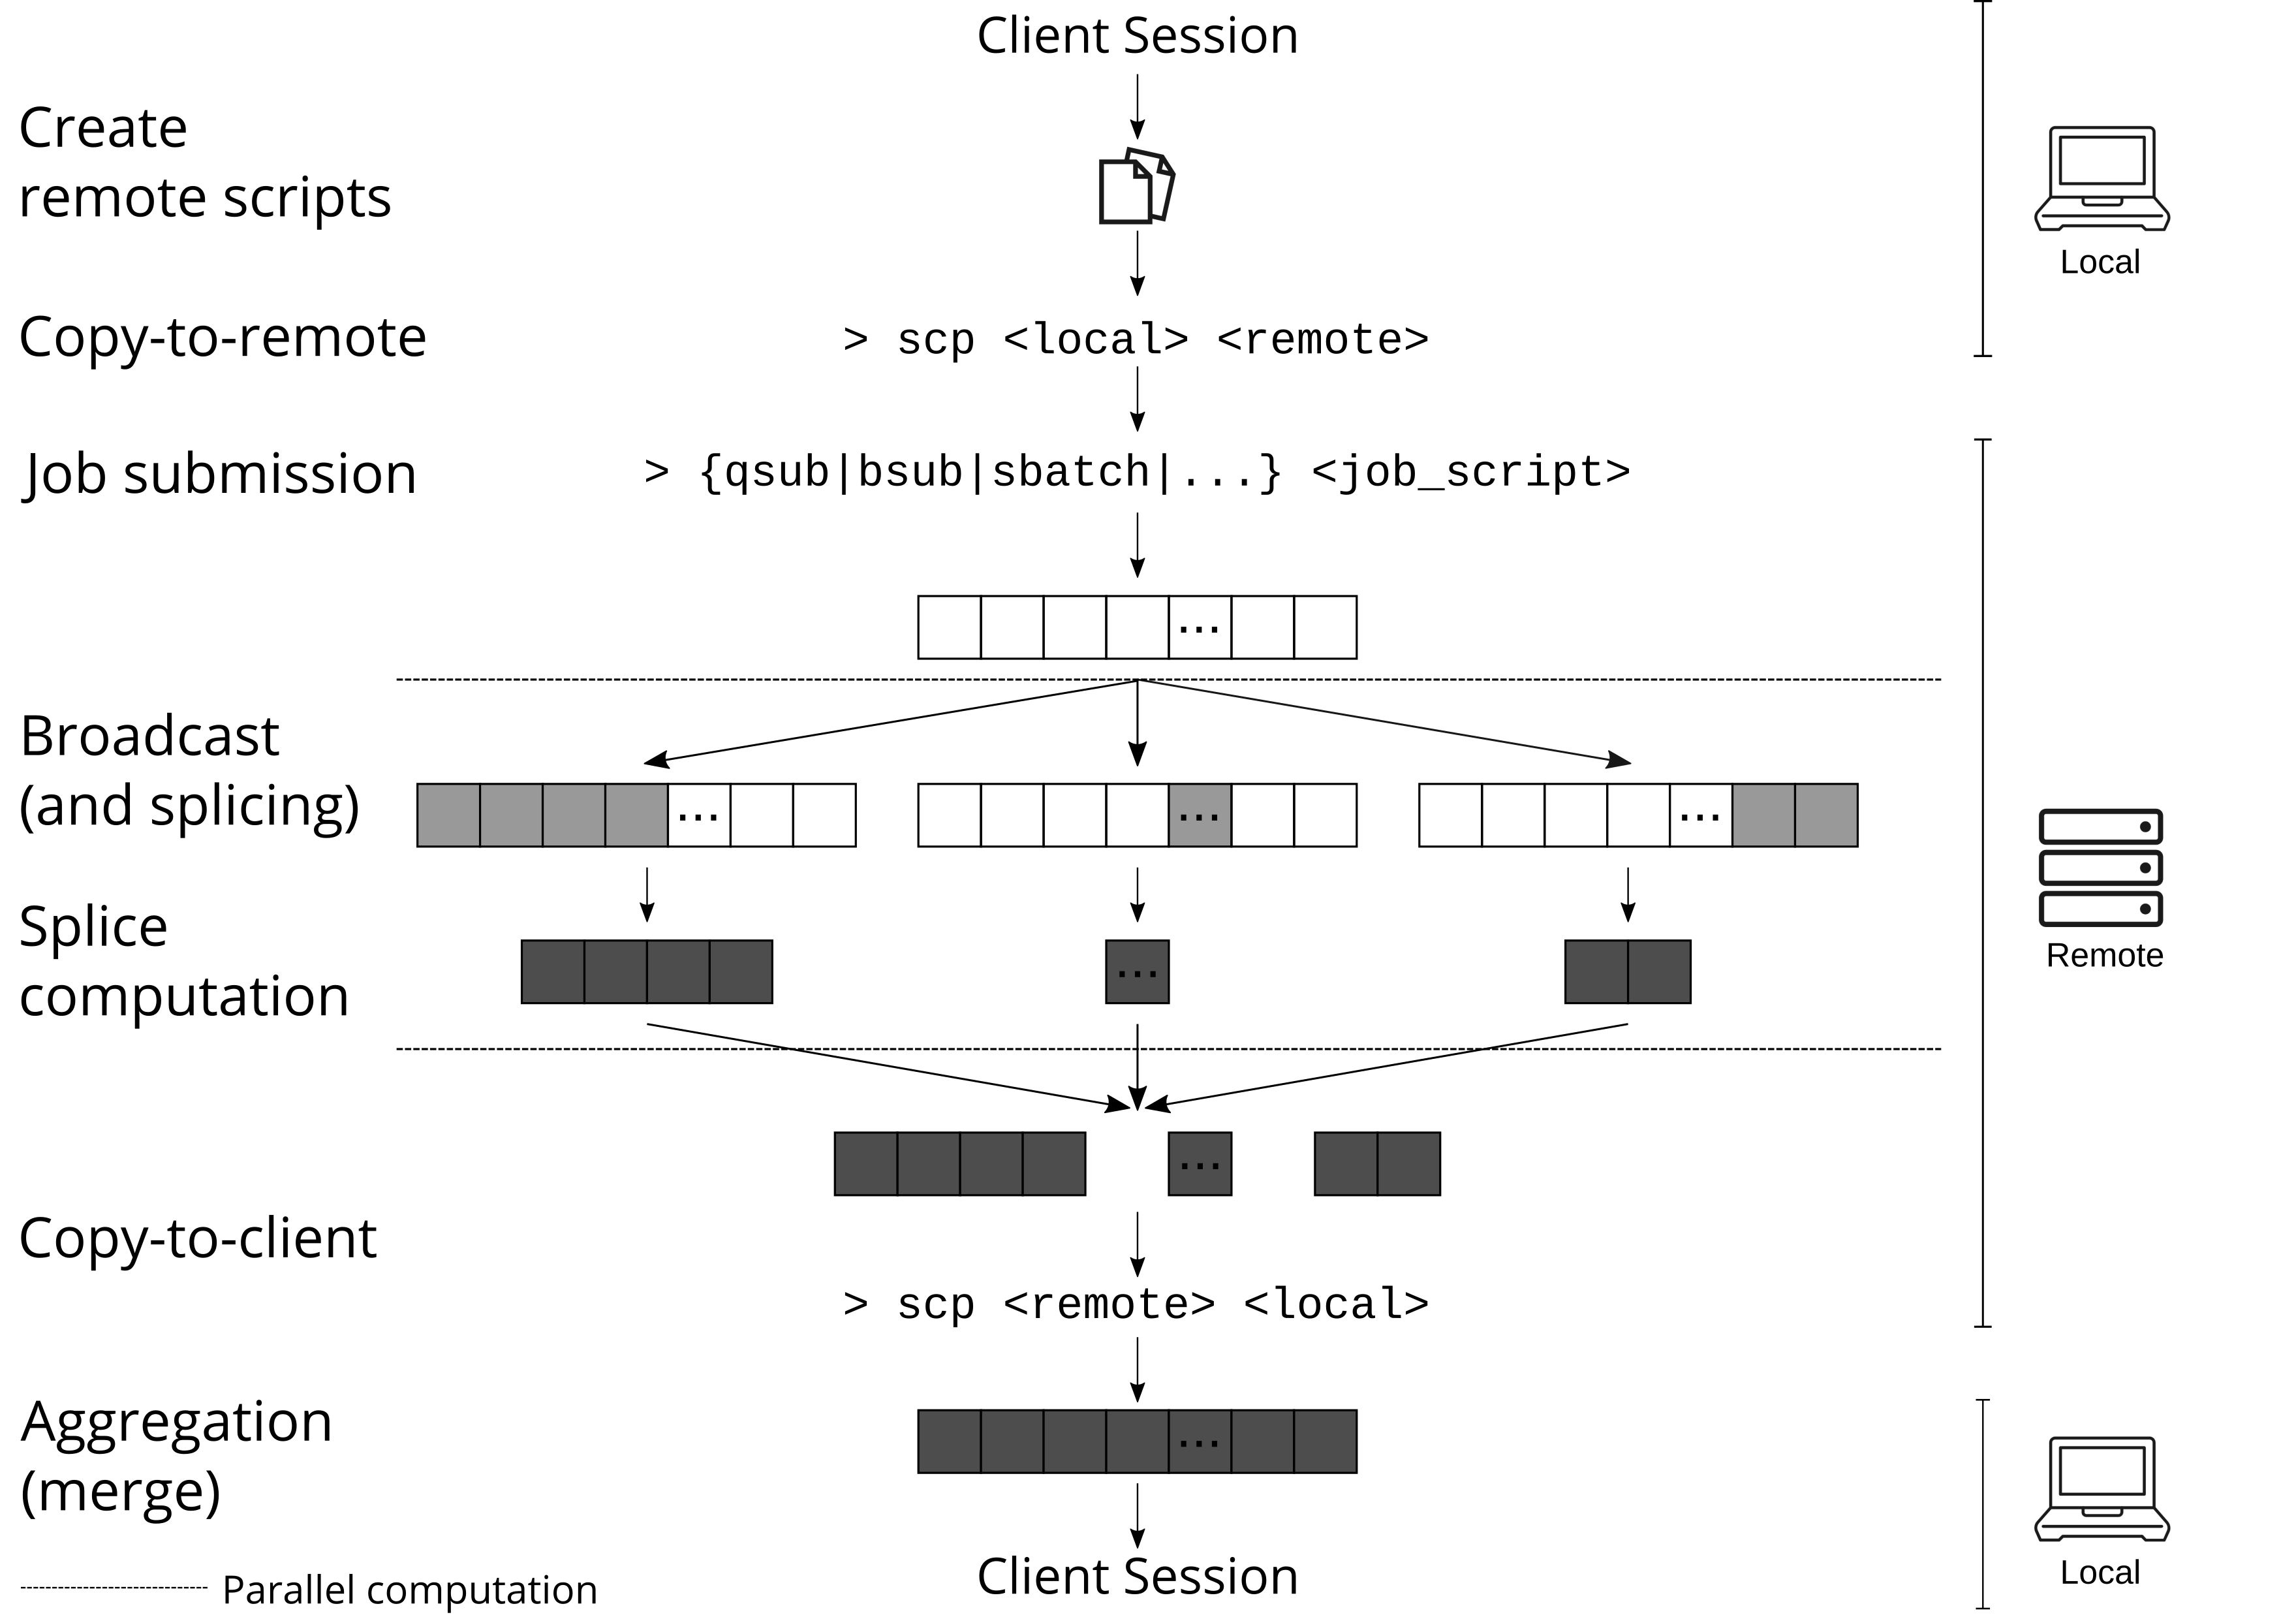
\includegraphics[width=0.95\textwidth]{ssh_dispatcher-third_step}
  }
\end{frame}

%----------------------------------------------------------------------------------------------------
\section{Components of a Dispatcher}
\begin{frame}[t]{Components of a Dispatcher unit}
  \small
  \only<1>{
    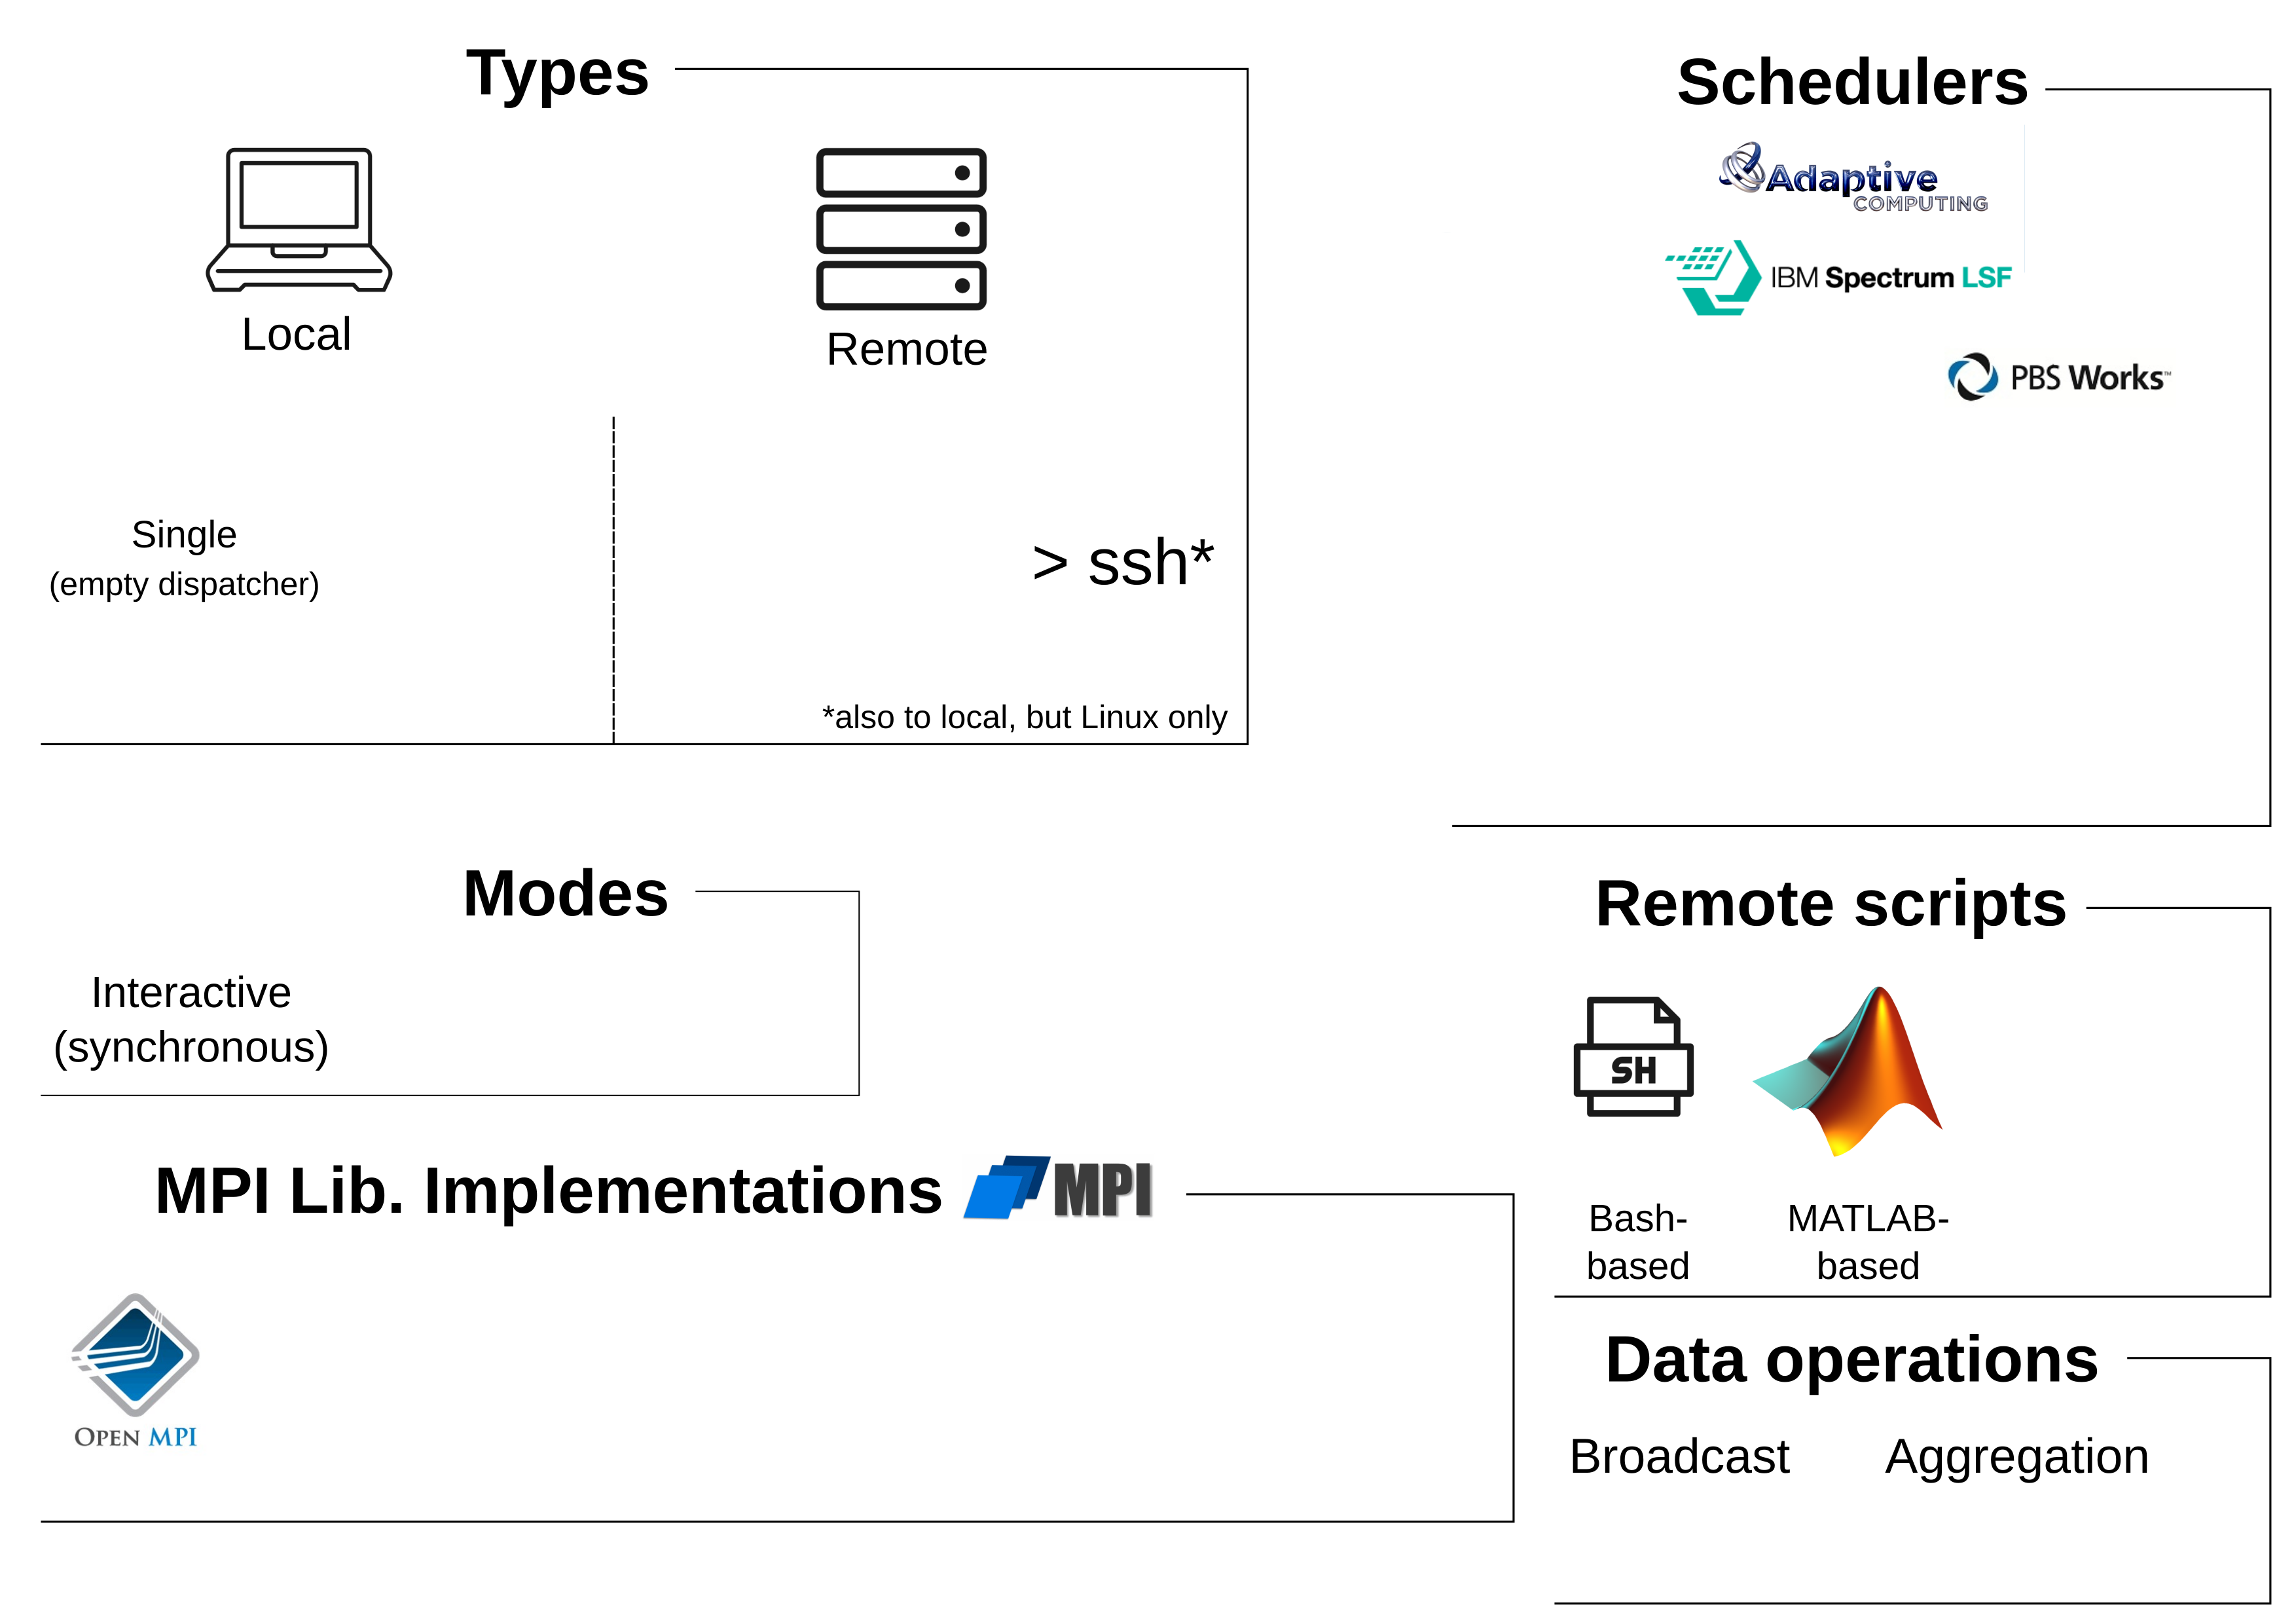
\includegraphics[width=0.95\textwidth]{uq_dispatcher_current}
  }
  \only<2>{
    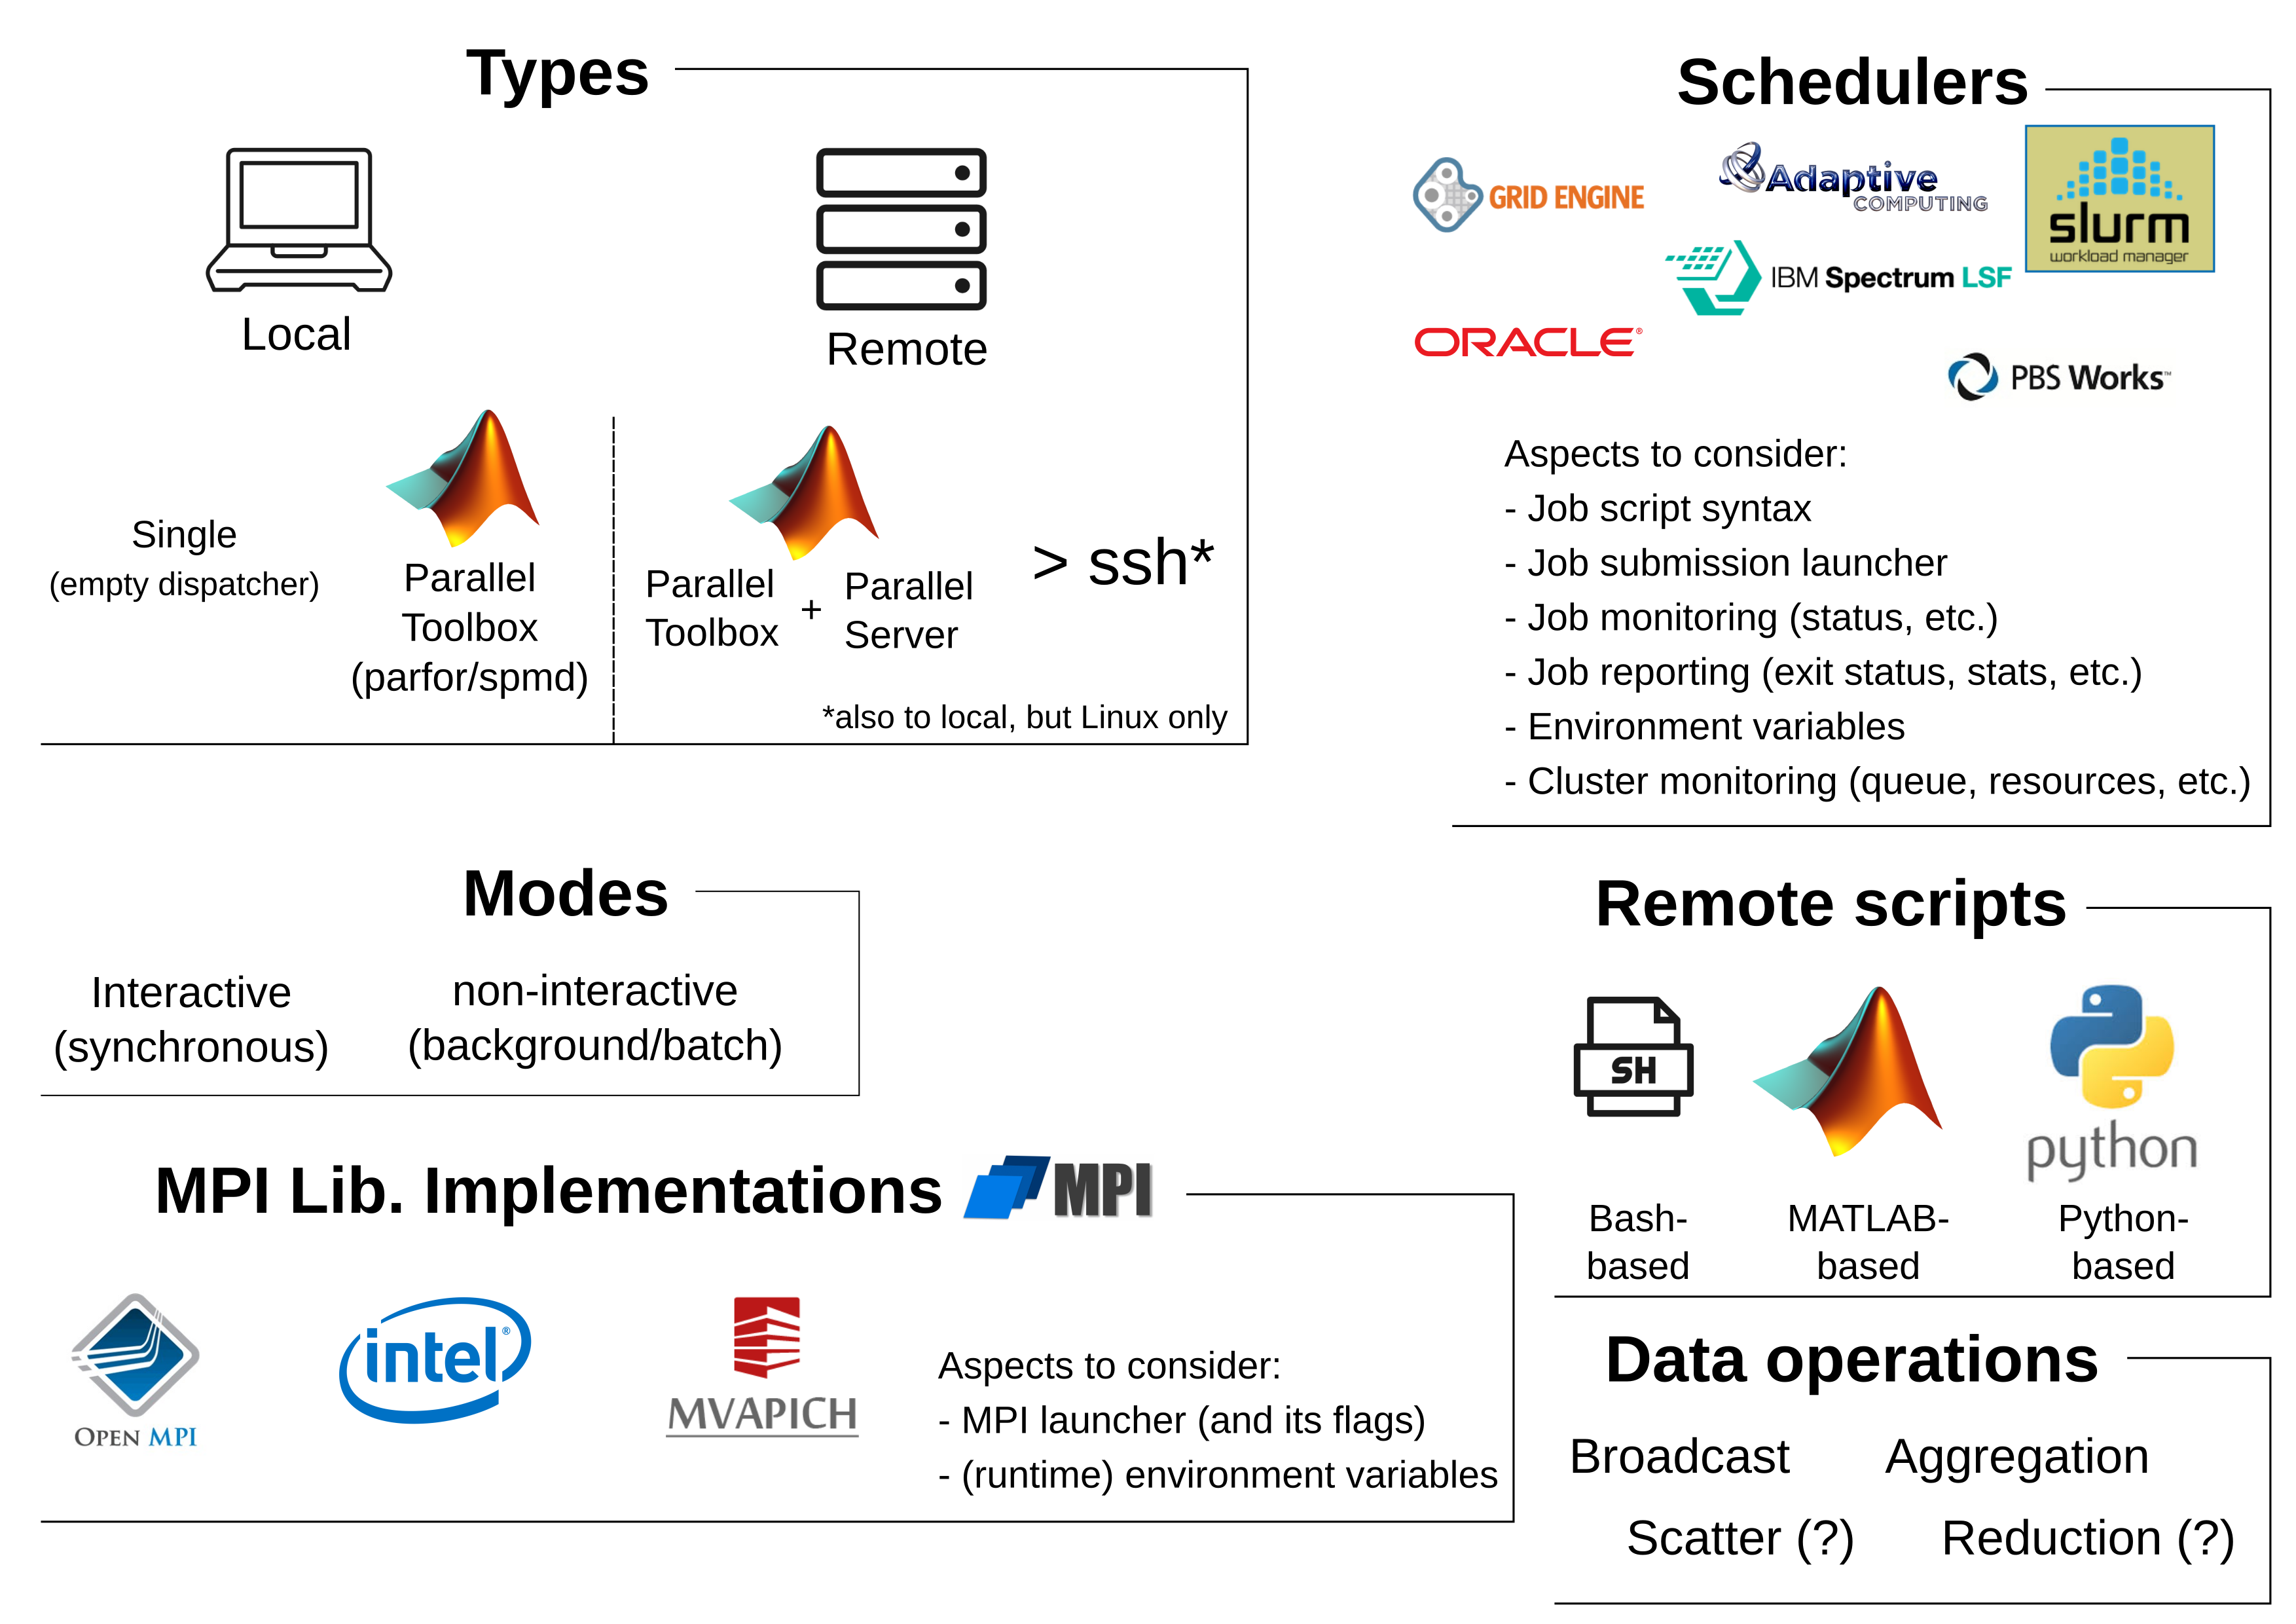
\includegraphics[width=0.95\textwidth]{uq_dispatcher}
  }
\end{frame}

%----------------------------------------------------------------------------------------------------
\begin{frame}[t]{Exploiting parallelisms for \uqlab{}}
  \small
  \Tit{Adaptive experimental design}
\end{frame}

%----------------------------------------------------------------------------------------------------

%----------------------------------------------------------------------------------------------------
\begin{frame}[t]{What's next?}
	\small
  \Tit{Challenges}
	\begin{columns}
		\begin{column}[T]{0.8\linewidth}
			\begin{itemize}
				\item SSE for surrogate modeling can be applied for {\altx 
				non-smooth} models and models with {\altx complex local 
				characteristics}
				\item SSE for Bayesian calibration requires an {\altx adaptive 
				experimental design} strategy
				\item {\altx Adaptive SSE} works for very peaked likelihood 
				functions with 
				{\altx 
				compact support}
				\item Only one tuning parameter ({\altx $\NRefine$})
				\item Analytical {\altx post-processing} capabilities are 
				extremely beneficial
			\end{itemize}
		\end{column}
		\begin{column}[T]{0.2\linewidth}
			\centering
		%	\includegraphics[width=\textwidth,trim={0 0 0 0.2cm},clip]{pros}
		\end{column}
	\end{columns}
	\vspace{4em}
	\begin{columns}
		\begin{column}[T]{0.2\linewidth}
		%	\includegraphics[width=\textwidth,trim={0 0 0 0.5cm},clip]{cons}
		\end{column}
		\begin{column}[T]{0.8\linewidth}
			\begin{itemize}
				\item At small experimental designs {\altx overfitting} is a 
				problem
				\item Requires relatively {\altx large experimental design}		
			\end{itemize}
		\end{column}
	\end{columns}
% logo placement
	\begin{tikzpicture}[overlay, remember picture] 
	\node at (current page.south east) 
	[
	anchor=south east,
	xshift=0mm,
	yshift=3mm
	] 
	{
	%	\includegraphics[width=0.14\textwidth]{uqlab}
	};
	\end{tikzpicture}
\end{frame}

\end{document}
